% define the type of document I want to make (article), set 12pt font and letter-sized paper
\documentclass[12pt, letterpaper]{article}
\usepackage[margin=1in]{geometry}
% the natbib package lets me use extra citation commands, authoryear sorts bibliography by author last name, then year of publication
\usepackage[authoryear]{natbib}
% the hyperref package lets me insert a hyperlink, and makes table of contents and references clickable
\usepackage{hyperref}
% graphicx allows....graphics
\usepackage{graphicx}
% letting LaTeX do line breaks easier so it doesn't complain about hboxes
\setlength{\emergencystretch}{5pt}


% enter the document environment to begin!
\begin{document}

% set the title
\title{Homework 5 - PHYS 5391}
% set author
\author{Elizabeth Vandegriff}
% set date as current date
\date{\today}

% make the above title/author/date visible
\maketitle
% leave the rest of the title page blank
\newpage


\section{Minimal Substorm Model}

Here we explore the occurrence of substorms over an entire year and attempt to quantify their frequency, what they may correlate with, and when they are most likely to occur.

\begin{figure}[!ht]
  \centering
  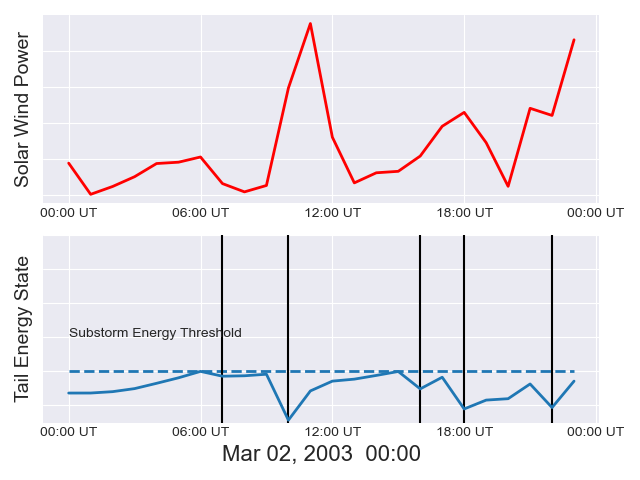
\includegraphics[width=10cm]{../imf20030302.png}
  \caption{Single day of data analyzed with minimal substorm model.}
  \label{fig:sub}
\end{figure}


We can examine each day's worth of data as individual plots, such in Fig. (\ref{fig:sub}), and if desired, we could make separate plots for each day of the year. However, this is not an effective way to examine the year as whole.

\begin{figure}[!ht]
  \centering
  \includegraphics[width=12cm]{../images/2003_substorm_hist.png}
  \caption{Number of substorms in each month.}
  \label{fig:hist}
\end{figure}

We can create a histogram of the number of substorms binned by month using the list of epochs that mark when a substorm occurs. We can plot this histogram to look for trends. Figure (\ref{fig:hist}) shows that most months have similar numbers of sumbstorms, with the average computed to be around 111.5 substorms monthly. In addition, we can calculate that the average weekly substorm frequency is about 25.7 and the average daily substorm frequency is about 3.7. One possible trend is that the number of substorms per month seem to decrease slightly from the beginning to the end of the year.

What if we look at the entire years' worth of data on a single plot?


\begin{figure}[!ht]
  \centering
  \includegraphics[width=12cm]{../images/2003_substorms_epochs.png}
  \caption{Plot showing all the substorms in a year}
  \label{fig:year}
\end{figure}

Figure (\ref{fig:year}) shows each substorm as a black line, which leaves us with a heavily saturated plot full of black lines! We can see qualitative information about frequency of substorms by visually examining the density of black lines, however this is not extremely helpful in our analysis.

But even in this plot, something else is hiding under the substorm lines...what if we remove the lines and simply look at the solar wind data and the energy calculation side by side?

\begin{figure}[!ht]
  \centering
  \includegraphics[width=12cm]{../images/2003_substorms.png}
  \caption{Comparison of solar wind data with the calculated energy.}
  \label{fig:yearcomp}
\end{figure}

Figure (\ref{fig:yearcomp}) shows a clear and consistent correlation between solar wind conditions and the energy, which is the determining factor for whether or not a substorm is occurring. In the daily plots, this relationship is not apparent at all, but when we look at the entire year plotted at once, we can see the obvious trend.

Because of the large spike toward the end of the plot, our axes are scaled down and hard to see, but we can zoom in to do a closer comparison.

\newpage

\begin{figure}[!ht]
  \centering
  \includegraphics[width=12cm]{../images/2003_substorms_cropped.png}
  \caption{Comparison of solar wind data with the calculated energy (cropped).}
  \label{fig:yearcrop}
\end{figure}

In Fig. (\ref{fig:yearcrop}), we can see slight differences between the data, but still extremely close correlation. Our final conclusion from this analysis is that substorm activity is directly tied to solar wind activity through the energy calculation. 

\end{document}
